\documentclass[12pt,letterpaper]{article}
\usepackage[utf8]{inputenx} %Codificacion del texto (ISO Latin1 encoding)

\usepackage{fancyhdr} %Permite acomodar a tu gusto la parte de arriba y
% abajo del documento
\usepackage[spanish]{babel} %Permite definir el idioma del dcumento
\usepackage{graphicx} %Permite exportar imagenes en formato eps
\usepackage{url} %Tipo de fuente para correos y paginas
\usepackage{pgf}
\usepackage{fleqn}
\usepackage{amssymb}
\usepackage{amsmath}
\usepackage{fancyvrb}
\usepackage{makeidx}
\usepackage{colortbl} %Permite colocar colores a las tablas
\usepackage{booktabs}
\usepackage[final]{pdfpages}
%%%%%%%%%%
%Margenes%
%%%%%%%%%%
\parskip 1mm %Espacio entre parrafos

\setlength{\topmargin}{0pt}
\topmargin      0.5cm
\oddsidemargin	0.1cm  % Ancho Letter 21,59cm
\evensidemargin 0.5cm  % Alto  Letter 27,81cm
\textwidth	17cm%15.5cm
\textheight	21.0cm
\headsep	4 mm
\parindent	0.5cm
%%%%%%%%%%%%%%%%%%%%%%
%Estilo del documento%
%%%%%%%%%%%%%%%%%%%%%%
\pagestyle{fancyplain}

%%%%%%%%%%%%%%%%%%%%%%%%%%%%%%%%%%%%%%%%%%%
%Fancyheadings. Top y Bottom del documento%
%%%%%%%%%%%%%%%%%%%%%%%%%%%%%%%%%%%%%%%%%%%
% Recuerde que en este documento la portada del documento no posee
% numeracion, pero de igual manera llamaremos a esa primera pagina la numero
% 1, y la que viene la dos. Esto es para tener una idea de las que
% llamaremos pares e impares
\lhead{Computación Científica 1} %Parte superior izquierda
\rhead{\bf \it Laboratorio I} %Parte superior derecha
\lfoot{\it } %Parte inferior izquierda. \thepage indica
% el numero de pagina
\cfoot{} %Parte inferior central
\rfoot{\bf \thepage} %Parte inferior derecha
\renewcommand{\footrulewidth}{0.4pt} %Linea de separacion inferior

\newcommand{\primaria}[1]{
	\textbf{\underline{#1}}
}

\newcommand{\foranea}[1]{
	\textbf{\textsl{#1}}
}

\newcommand{\primyfor}[1]{
	\underline{\foranea{#1}}
}

\makeatletter
\newcommand\subsubsubsection{\@startsection {paragraph}{1}{\z@}%
                                   {-3.5ex \@plus -1ex \@minus -.2ex}%
                                   {1.5ex \@plus.2ex}%
                                   {\normalfont\bfseries}}
\newcommand\subsubsubsubsection{\@startsection {subparagraph}{1}{\z@}%
                                   {-3.5ex \@plus -1ex \@minus -.2ex}%
                                   {1.5ex \@plus.2ex}%
                                   {\normalfont\bfseries}}


\makeatother
 

\begin{document}
\title{Computaci\'on Científica I \\ \begin{Large}Laboratorio 1\end{Large}} 
\author{Victor Gonzalez Rodriguez\\victor.gonzalezr@usm.cl - 2.773.029-9}
\date{14 de mayo de 2012}
\maketitle


\section{Benchmark de multiplicaciones}
\begin{itemize}
\item \textbf{Software:} Para desarrollar el programa que realiza el benchmark comparativo, se ocupó la librería \textit{numpy}, para el manejo mejorado de matrices y arrays. Cada una de las funciones de multiplicación, ejecuta un proceso atómico de multiplicaciones para asi comparar de mejor manera cuanto demora cada método.
\item \textbf{Conclusiones:} A partir de las comparaciones hechas entre los distintos métodos usando las matrices propuestas, se ha logrado concluir que el método más eficiente para calcular la multiplicación entre 2 matrices, es el de enfoque fila, seguido por el enfoque columna, y finalmente el producto punto, siento notablemente más lento que los otros métodos.\\\\
En el siguiente resultado de ejemplo, el producto punto llega a ser 20 veces mas lento que el enfoque fila:
\begin{verbatim}
Producto punto:		1.66762685776  segundos.
Enfoque Columna:	0.0907769203186  segundos.
Enfoque Fila:		0.0868830680847  segundos.
\end{verbatim}
\end{itemize}

\section{Tipos de matriz}
\begin{itemize}
\item \textbf{Software:} Para el desarrollo del software que analiza que tipo de matriz es una matriz A, se utilizó principalmente la libreria \textit{numpy} y sus habilidades de computo de álgebra lineal \textit{numpy.linalg} (para calcular la inversa, la conjugada de una matriz, etc.).
\item \textbf{Conclusiones:} Fue interesante descubrir las propiedades que cumplen los tipos de matrices y como ayudan a determinar ciertos comportamientos y propiedades que pueden ayudar a simplificar el cálculo.
\end{itemize}

\section{Transformación de imágenes}
\begin{itemize}
\item \textbf{Software:} Para este software se usó la libreria \textit{numpy}, \textit{scipy} y \textit{pylab}.\\
Las funciones generan matrices (imágenes), las cuales se adaptan a la transformación aplicada, por lo que no importa que tan rebuscada es la transformación, siempre se generará una imagen correcta de salida.
\item \textbf{Conclusiones:} Se puede decir que son transformaciones lineales, porque nunca una transformación me llevó a poner 2 veces un valor en el mismo pixel (elemento de la matriz). Además esto se puede ver claramente al notar que las matrices resultantes no aparecen con filas desaparecidas.s
\end{itemize}

\section{Gráfica de vectores}
\begin{itemize}
\item \textbf{Software:} En el desarrollo del software para la gráfica de vectores, se utilizaron las librerías \textit{numpy}, \textit{pylab} y otras funciones estándar de Python. \textit{Numpy} se ocupo para aprovechar sus capacidades de manejo de matrices y arrays, y \textit{pylab} para poder mostrar un gráfico.\\
Las funciones ejecutan algoritmos lo más atómicos posibles, para asi evitar tiempo innecesario de cómputo.\\
Para le obtención de vectores aleatorios, se ocupan números entre -10 y 10, para así evitar números excesivamente grandes o números excesivamente pequeños, ya que la funcion \textit{random()} solo genera valores entre 0 y 1, y la función \textit{numpy.empty()}, entrega valores excesivamente peqeños.
\item \textbf{Conclusiones:} Luego de ir probando con distintos valores, se puede notar, que entre más grande es el número de vectores, se vá generando la forma de un círculo, con un radio \textit{norm}. Esto es congruente con la forma de las p-normas con p=2, la cual es un círculo de radio 1.\\
Acá con un ejemplo con n=1000 y norm = 2:\\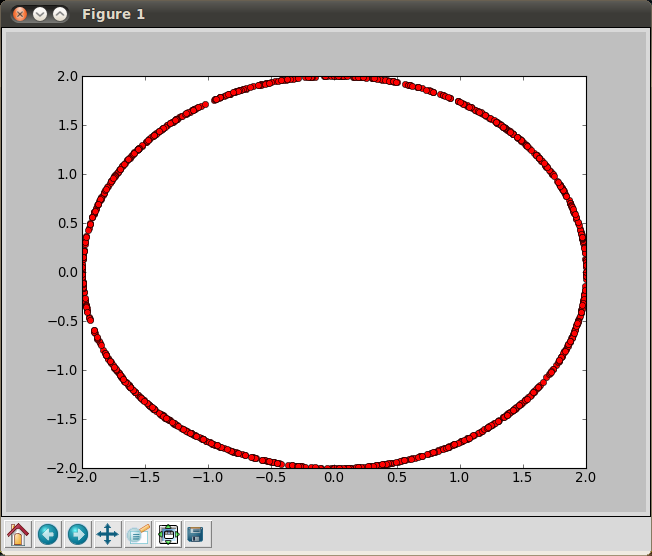
\includegraphics[width=10cm]{norm.png}

\end{itemize}
\end{document} 